\documentclass[10pt,addpoints]{exam}
\usepackage[utf8]{inputenc}
\usepackage[spanish,es-noshorthands]{babel}
\usepackage{hyperref}
\usepackage{amsmath}
\usepackage{amsfonts}
\usepackage{amssymb}
\usepackage{graphicx}
\usepackage{tikz}
\usepackage{multicol}
\usepackage[papersize={5.5in,8.5in},top=.75cm,bottom=.75cm,left=.75cm,right=.75cm]{geometry}
\printanswers
\begin{document}
\title{\begin{minipage}{.2\textwidth}
        
\includegraphics[height=1.75cm]{Images/logo-colegio.png}
       \end{minipage}
\begin{minipage}{.55\textwidth}
 \begin{center}
Pre-Saber 2014, Form A\\Matemáticas $11^{\circ}$
\end{center}
\end{minipage}
\begin{minipage}{.2\textwidth}

\includegraphics[height=1.75cm]{Images/logo-sed.png} 
\end{minipage}
}
\author{Germ\'{a}n Avendaño Ram\'{i}rez~\thanks{Lic. Matemáticas U.D., M.Sc. U.N.}}
\date{}
\maketitle
\begin{center}
\fbox{\fbox{\parbox{\textwidth}{\centering
\textit{Conteste en su cuaderno haciendo las justificaciones necesarias. Esta prueba se revisará en la siguiente clase}}}}
\end{center}
\begin{questions}
\question El caudal ($Q$) se define como el volumen de algún líquido que pasa por un conducto en un determinado tiempo
\[Q=\dfrac{V}{t}\]
Donde $V$ es el volumen del líquido y $t$ es el tiempo que tarda en pasar.
De acuerdo con esto, una unidad de medida del caudal de líquido puede ser

\begin{oneparchoices}
\choice $\dfrac{m^{3}}{litro}$
\choice $\dfrac{km}{hora}$
\choice $\dfrac{litro}{dm}$
\CorrectChoice $\dfrac{cm^{3}}{seg}$
\end{oneparchoices}
\question En la figura se representa el plano del primer piso de un edificio, conformado por cuatro apartamentos de igual forma y medida que comparten un espacio común de forma cuadrada donde se encuentra una escalera.
\begin{center}
\begin{tikzpicture}[scale=1.9]
\shadedraw (0,0) rectangle (6,2);
\draw (3,0)--(3,0.6);
\draw (3,1.4)--(3,2.0);
\draw (3.4,1)--(6,1);
\draw (0,1)--(2.6,1);
\filldraw[fill=white] (2.6,0.6) rectangle node {Escalera} (3.4,1.4);
\node (Ap3) at (1.5,.5) {Apartamento 3};
\node (Ap1) at (1.5,1.5) {Apartamento 1};
\node (Ap2) at (4.5,1.5) {Apartamento 2};
\node (Ap4) at (4.5,.5) {Apartamento 4};
\node (x) at (6.2,1.5) {$x$};
\draw[|-|] (6.1,1)--(6.1,2);
\draw[|-|] (3,2.1)--(6,2.1);
\node (y) at (4.5,2.2) {$y$};
\draw[|-|] (2.6,.5)--(3.4,.5);
\node (x-2) at (3,0.4) {$x-2$};
\end{tikzpicture}
\end{center}
¿Cuál de las siguientes expresiones representa el área total de los 4 apartamentos (área sombreada)?

\begin{oneparchoices}
\choice $4xy-x+2$
\CorrectChoice $4xy-(x-2)^{2}$
\choice $2xy-(x-2)^{2}$
\choice $2xy-x+2$
\end{oneparchoices}
\question La siguiente tabla muestra, para tres años consecutivos, el valor del auxilio de transporte mensual que reciben los trabajadores de una empresa y el promedio de la tarifa de un pasaje para el servicio de transporte urbano en la ciudad:
\begin{center}
\begin{tabular}{|c|c|c|}
\hline 
Año & Auxilio de Transporte (mensual) & Tarifa de un pasaje (promedio) \\ 
\hline 
2009 & \$59.300 & \$1.500 \\ 
\hline 
2010 & \$61.500 & \$1.600 \\ 
\hline 
2011 & \$63.800 & \$1.700 \\ 
\hline 
\end{tabular} 
\end{center}
Si un trabajador debe comprar al mes 40 pasajes, se puede afirmar que, con respecto al primer año, en el tercero el desequilibrio (el costo de transporte que no le cubre el auxilio) es:
\begin{choices}
\begin{multicols}{2}
\choice Mayor en \$200
\choice Menor en \$4.300
\choice 3 veces mayor
\CorrectChoice 6 veces mayor
\end{multicols}
\end{choices}
\question Dada una recta $m$ y un punto $P$ cualquiera, es posible trazar una recta paralela a la recta $m$ que pase por el punto $P$, siguiendo siete pasos.
\begin{enumerate}
\item Se marca un punto $Q$ cualquiera en la recta $m$.
\item Se traza el segmento $QP$
\item Se traza la circunferencia $j$ de centro $Q$ y radio de la longitud de $QP$ que interseca a la recta $m$ en $R$ y $R'$.
\item Se traza la circunferencia $k$ con centro en $P$ y radio de la longitud de $QP$.
\item Se traza la circunferencia $l$ con centro en $Q$ y radio $RP$ que interseca la circunferencia $k$ en los puntos $S$ y $T$
\item Se traza la recta $n$ que pasa por los puntos $P$ y $S$.
\item Como el ángulo $RQP$ es congruente con el ángulo $QPS$, las rectas $m$ y $n$ son paralelas.
\end{enumerate}
La figura que muestra correctamente la construcción geométrica descrita es
\begin{choices}
\begin{multicols}{2}
\CorrectChoice 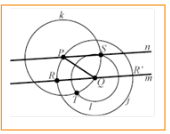
\includegraphics[scale=.65]{Images/Pantallazo-41.png} 
\choice 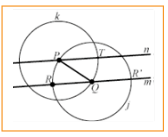
\includegraphics[scale=.65]{Images/Pantallazo-42.png} 
\choice 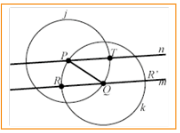
\includegraphics[scale=.65]{Images/Pantallazo-43.png} 
\choice 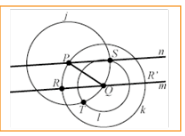
\includegraphics[scale=.65]{Images/Pantallazo-44.png} 
\end{multicols}
\end{choices}
\uplevel{
RESPONDA LAS PREGUNTAS \ref{q1} y \ref{q2} DE ACUERDO CON LA SIGUIENTE INFORMACIÓN.
\begin{center}
\begin{tabular}{|p{.45\textwidth}|p{.45\textwidth}|}
\hline 
Opción 1 & Opción 2 \\ 
\hline 
1. Dividen \$20.000 entre 3. & 1. Cada uno halla el cociente del costo de su pedido entre el precio total de los pedidos. \\ 
2. Cada uno multiplica el costo de su pedido por 1,1. & 2. Cada uno paga el producto de multiplicar el
cociente hallado en el paso 1 por el monto total
de la cuenta. \\ 
3. Cada uno paga la suma del valor obtenido en 2 y el
obtenido en 1. &  \\ 
\hline 
\end{tabular} 
\end{center}
}
\question \label{q1} El mesero que los oye discutir sobre las opciones, les dice que quien haga el pedido más barato siempre pagará menos con la opción 2 que con la opción 1. Esta afirmación es correcta porque:
\begin{choices}
\choice En la opción 1, se multiplica por 1,1 el precio de los pedidos de manera que resulta un 10\% más alto frente a la opción 2.
\CorrectChoice En la opción 2, el valor que paga cada persona por la reserva es proporcional al valor de su pedido; no es un valor fijo.
\choice En la opción 1, se suman valores adicionales a aquellos que incluye la opción 2 y por lo tanto resulta más alto el valor a pagar.
\choice En la opción 2, el repartir proporcionalmente la cuenta hace que el pago de la reserva sea igual para todos.
\end{choices}
\question \label{q2} Uno de los amigos plantea una nueva opción:

OPCIÓN 3
\begin{enumerate}
\item Cada uno calcula a qué porcentaje del valor total de lo consumido corresponde el valor de lo que él pidió.
\item Cada uno multiplica el porcentaje obtenido en 1 por los \$20.000 de la reserva.
\item Cada uno multiplica el porcentaje obtenido en 1 por el valor total de la propina.
\item Cada uno paga la suma del valor de lo que pidió con los valores obtenidos en los pasos 2 y 3.
\end{enumerate}
Él afirma que este procedimiento es mejor para quien haga el pedido más barato, en comparación con los procedimientos de las opciones 1 o 2. Sin embargo, dicha afirmación es incorrecta porque:
\begin{choices}
\choice La opción 1 es equivalente a la opción 3 pues en las dos se divide el valor de la reserva en partes iguales entre los amigos.
\CorrectChoice La opción 2 es equivalente a la opción 3 pues en ambos casos se calcula la cuenta de cada uno proporcionalmente al valor de su pedido.
\choice La opción 1 es equivalente a la opción 3 pues tanto en una como en otra, los pasos iniciales establecen el valor a pagar por la reserva y la propina.
\choice La opción 2 es equivalente a la opción 3 pues en el primer paso de la opción 3 el porcentaje obtenido es igual al cociente obtenido en el primer paso de la opción 2.
\end{choices}
\question Se lanzan 2 dados y se considera la suma de los puntajes obtenidos. La tabla muestra las parejas posibles para algunos puntajes.
\uplevel{
\begin{center}
\begin{tabular}{|c|p{6cm}|p{2.1cm}|}
\hline 
\textbf{Pun-} & \qquad \textbf{Parejas} & \textbf{\# de}\\ 
\textbf{taje} & \qquad \textbf{posibles} & \textbf{posibilidades}\\ \hline
2 & (1,1) & \hspace*{1cm}1 \\ 
\hline 
3 & (1,2), (2,1) & \hspace*{1cm}2 \\ 
\hline 
4 & (1,3), (2,2), (3,1) & \hspace*{1cm}3 \\ 
\hline 
5 & (1,4), (2,3), (3,2), (4,1) & \hspace*{1cm}4 \\ 
\hline 
6 & (1,5), (2,4), (3,3), (4,2), (5,1) & \hspace*{1cm}5 \\ 
\hline 
7 & (1,6), (2,5), (3,4), (4,3), (5,2), (6,1) & \hspace*{1cm}6 \\ 
\hline 
\end{tabular} 
\end{center}
}
Si se lanzan dos veces los 2 dados, ¿cuántas posibilidades hay de obtener 10 puntos en total, de manera que en el primer lanzamiento se obtengan 6 puntos?

\begin{oneparchoices}
\choice 8
\CorrectChoice 15
\choice 16
\choice 24
\end{oneparchoices}
\question Un colegio necesita enviar 5 estudiantes como representantes a un foro sobre la contaminación del medio ambiente. Se decidió que 2 estudiantes sean de grado décimo y 3 de grado undécimo. En décimo hay 5 estudiantes preparados para el foro y en undécimo hay 4. ¿Cuántos grupos diferentes pueden formarse para enviar al foro?

\begin{oneparchoices}
\choice 9
\CorrectChoice 14
\choice 20
\choice 40
\end{oneparchoices}
\uplevel{PREGUNTA ABIERTA}
\question La figura muestra la suma de los ángulos internos en diferentes polígonos regulares.
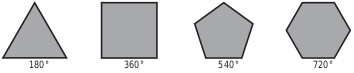
\includegraphics[scale=.5]{Images/Pantallazo-45.png} 
Debido a las propiedades de los polígonos regulares, es posible demostrar que el resultado de cada suma se traduce en la expresión $180\times (n-2)$ ¿Qué representa $n$ en cada polígono?
%\answerline
\end{questions}
%cuadro de puntajes
%\begin{center}
%\gradetable[h][pages]
%\end{center}
\end{document}